\documentclass[12pt,a4paper,oneside]{scrreprt}
\usepackage{fontspec}
\setmainfont{Latin Modern Roman}
\usepackage[ngerman]{babel}
\usepackage{graphicx}
\usepackage{booktabs}
\usepackage{csquotes}
\usepackage[backend=biber,style=numeric,sorting=none]{biblatex}
\addbibresource{literatur.bib}
\usepackage[hidelinks]{hyperref}
% Hier eure Angaben eintragen. Sonderzeichen wie & als \& schreiben.
\newcommand{\Arbeitstitel}{Entwicklung eines Systems zur Meldung und Verwaltung gefundener Gegenstände}
\newcommand{\Team}{Georg Fischinger \\ Fabian Grasböck \\ David Dammerer}
\newcommand{\Betreuung}{Namen der betreuenden Lehrpersonen}
\newcommand{\Schuljahr}{2026/27}
\newcommand{\Abgabedatum}{5. April 2027}

\begin{document}
\begin{titlepage}
\centering
{\Large HTBLuVA Salzburg\par}
\vspace{2cm}
{\huge\bfseries Diplomarbeit\par}
\vspace{1cm}
{\LARGE \Arbeitstitel\par}
\vspace{2cm}
{\large \Team\par}
\vfill
Betreuung: \Betreuung\par
Schuljahr: \Schuljahr\par
Abgabe: \Abgabedatum
\end{titlepage}
\pagenumbering{roman}
\chapter*{Kurzfassung}
\addcontentsline{toc}{chapter}{Kurzfassung}
Hier Problem, Ziel, Vorgehen und Ergebnis kurz zusammenfassen.
\chapter*{Abstract}
\addcontentsline{toc}{chapter}{Abstract}
The project aims to develop a lost-and-found system for the HTL Salzburg. It combines a web application, database, and a hardware terminal with an integrated locking mechanism. Users will be able to report, search, and manage lost and found items more efficiently. The project covers database design, system architecture, user interface development, and hardware integration. The goal is to create a secure, user-friendly, and fully functional prototype that simplifies the management and return of lost items.
\tableofcontents
\clearpage
\pagenumbering{arabic}
% !TeX root = ../main.tex
\chapter{Einleitung}\label{chap:einleitung}
\section{Ausgangslage}
Beschreibt das konkrete Problem und die Zielgruppe.
\section{Zielsetzung und Abgrenzung}
Was soll entstehen? Welche Fragen beantwortet die Arbeit?
\section{Aufgabenverteilung}
Welche Person verantwortet welchen Teil?

\begin{figure}
    \centering
    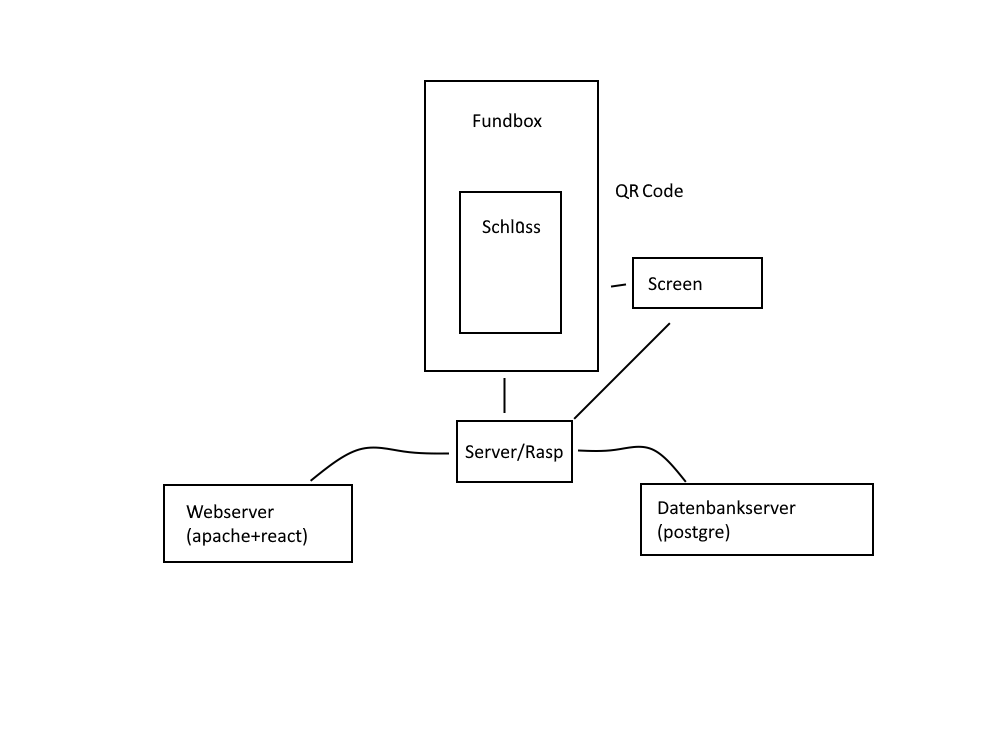
\includegraphics[width = 0.5\textwidth]
    {bilder/Components1.png}
    \caption{Komponentendiagramm}
    \label{fig.componentDiagram}
\end{figure}

% !TeX root = ../main.tex
\chapter{Grundlagen}\label{chap:grundlagen}
Belegt fachliche Aussagen mit passenden Quellen. Ein Beispiel für einen
Quellenverweis auf die LaTeX-Projektseite: \autocite{latexproject}.
Die Quelle dient hier nur als Syntaxbeispiel, nicht als Beleg für eure Fachthemen.
\section{Begriffe}
Definiert die für eure Arbeit wichtigen Begriffe.

% !TeX root = ../main.tex
\chapter{Anforderungen und Konzept}
\section{Anforderungen}
\begin{table}[htbp]
\centering
\begin{tabular}{lll}
\toprule
ID & Anforderung & Prüfkriterium \\
\midrule
A01 & Daten speichern & Datensatz nach Neustart vorhanden \\
\bottomrule
\end{tabular}
\caption{Beispiel einer Anforderung}\label{tab:anforderungen}
\end{table}
Auf Tabelle~\ref{tab:anforderungen} wird automatisch verwiesen.
\section{Gesamtablauf und Schnittstellen}
Beschreibt Datenfluss, Zuständigkeiten und Integration.


% !TeX root = ../main.tex
\chapter{Umsetzung: Teil von Person A}
\section{Entwurf}
Beschreibt und begründet eure Entscheidungen.
\section{Implementierung}
Erklärt die Umsetzung mit ausgewählten Beispielen.

% !TeX root = ../main.tex
\chapter{Umsetzung: Teil von Person B}
\section{Entwurf}
Beschreibt und begründet eure Entscheidungen.
\section{Implementierung}
Erklärt die Umsetzung mit ausgewählten Beispielen.

% !TeX root = ../main.tex
\chapter{Umsetzung: Teil von Person C}
\section{Entwurf}
Beschreibt und begründet eure Entscheidungen.
\section{Implementierung}
Erklärt die Umsetzung mit ausgewählten Beispielen.

% !TeX root = ../main.tex
\chapter{Testing und Evaluation}
\section{Testplan und Testfälle}
Dokumentiert Ausgangslage, Schritte, Soll-Ergebnis und Ist-Ergebnis.
\section{Integrationstest}
Prüft den vollständigen Ablauf über alle Komponenten hinweg.
\section{Evaluation und Verbesserungen}
Beschreibt Methode, Ergebnisse, Grenzen und daraus abgeleitete Änderungen.

% !TeX root = ../main.tex
\chapter{Fazit und Ausblick}
Welche Ziele wurden erreicht? Was bleibt offen?

\printbibliography[heading=bibintoc,title={Literaturverzeichnis}]
\appendix
% !TeX root = ../main.tex
\section{Beispieldatensatz für das Fundsachensystem}
Die folgende Tabelle enthält zufällig zusammengestellte Beispieldaten zur
Veranschaulichung der Erfassung und Verwaltung von Fundgegenständen. Sie stellt
keine tatsächlichen Meldungen oder Evaluationsergebnisse dar.

\begin{table}[htbp]
    \centering
    \caption{Beispielhafte Fundgegenstände und Bearbeitungsstatus}
    \label{tab:fundgegenstaende-beispiel}
    \begin{tabular}{llll}
        \toprule
        Gegenstand & Kategorie & Fundort & Status \\
        \midrule
        Schwarze Trinkflasche & Trinkflasche & Turnsaal & Abholbereit \\
        Blaues Federpennal & Schulsachen & Raum B204 & Nicht zugeordnet \\
        Grauer Regenschirm & Kleidung/Zubehör & Haupteingang & Abgeholt \\
        Roter USB-Stick & Elektronik & Bibliothek & In Verwahrung \\
        Grüne Sporttasche & Tasche & Garderobe & Abholbereit \\
        \bottomrule
    \end{tabular}
\end{table}
\chapter{Ergänzende Materialien}
Hier können Testprotokolle, Fragebögen oder ergänzende Angaben stehen.

\end{document}
